\subsection{Part 2 measured outcomes}
All sixteen full episodes pass independent action/monitor replay, source/checkpoint
and native sampling-seed checks. Safe completion is 3/4 for A, B and D and 2/4 for C;
each condition has one violating episode (Figure~\ref{fig:part2-outcomes}). Requested
completion is 3/4 in every condition. A/B/D each have one unsafe unfinished episode;
C has one unsafe completion and one safe unfinished episode. All conditions safely
complete both task 0010 episodes. On task 0039, A/B/D each safely complete one of two,
whereas C safely completes neither. These small descriptive counts support no claim
that one schedule is superior or that frequent feedback itself causes harm.

\begin{figure*}[t]
\centering
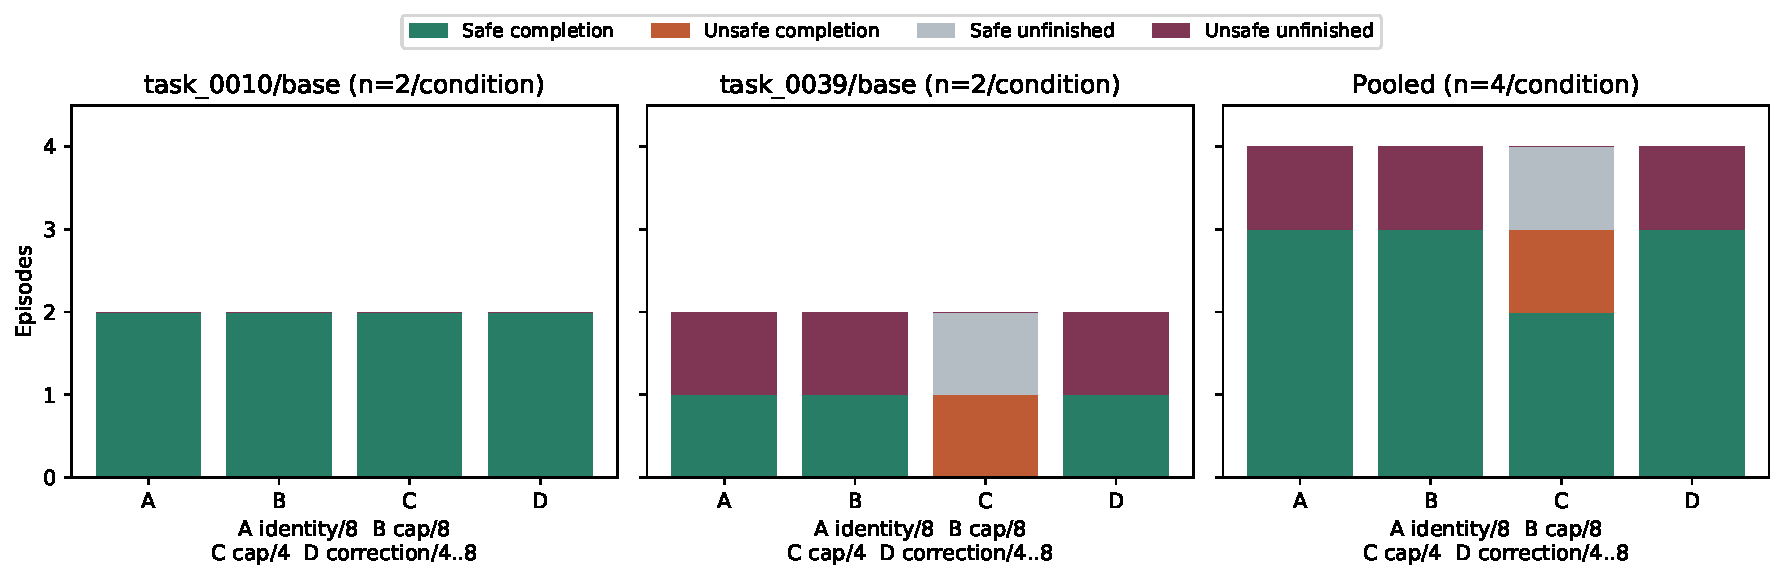
\includegraphics[width=\textwidth]{part2-outcomes.pdf}
\caption{Part 2's complete sixteen-episode sample, with unsafe completion and both
unfinished categories preserved. Each scene has two episodes per condition; pooled
denominators are four. A is identity/8, B is cap/8, C is cap/4 and D is correction/4--8.}
\Description{Pooled safe completions are three, three, two and three of four.
Every condition has one violating episode; only C completes unsafely.}
\label{fig:part2-outcomes}
\end{figure*}

The adaptive rule never changes the query schedule: every one of D's 337 actual
inter-query intervals is eight actions (Figure~\ref{fig:part2-feedback}). Its correction
threshold is crossed once, at action eight, when a query is already due. There is no
crossing at actions four through seven. Its largest accumulated correction is .60146.
Thus this run supplies no adaptive-feedback gain while leaving an actively triggering
rule untested. The threshold is retained rather than adjusted against these outcomes.
C uses 750 queries versus B's 336 without improving measured safe completion.

\begin{figure*}[t]
\centering
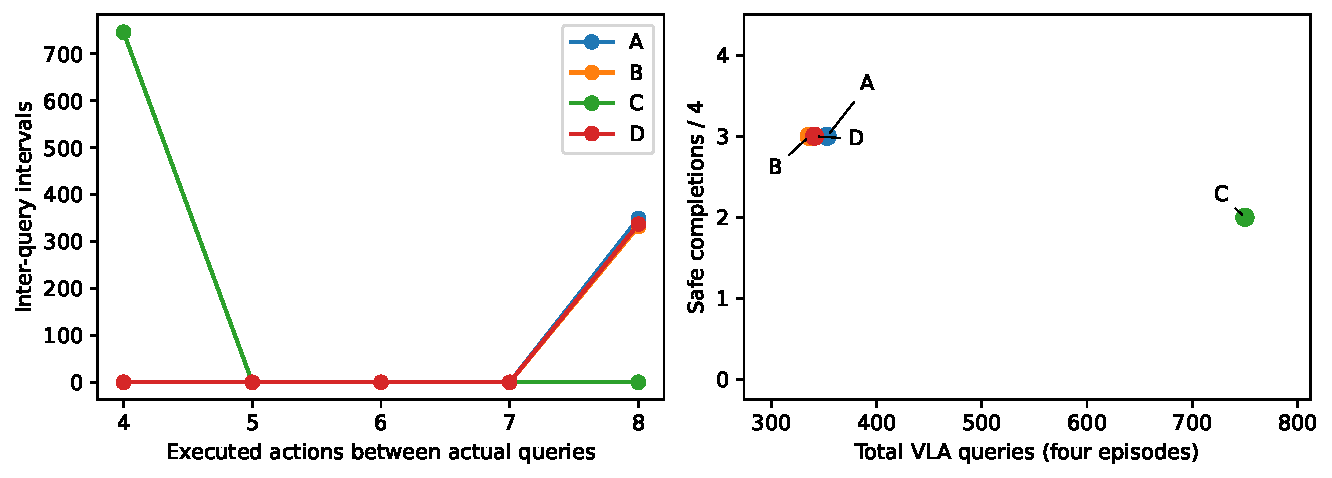
\includegraphics[width=.85\textwidth]{part2-feedback.pdf}
\caption{Observed inter-query intervals and query cost in Part 2. A/B/D always wait
eight actions; C always waits four. Safe completions have denominator four.}
\Description{The adaptive controller D shares the fixed-eight schedule, while fixed
four more than doubles queries without increasing safe completions.}
\label{fig:part2-feedback}
\end{figure*}

\begin{table}[t]
\caption{Part 2 costs. Time is measured inside each evaluator, including capture;
outer process time over all sixteen episodes is 1,897.69 s.}
\label{tab:part2-costs}
\begin{tabular}{lrrrr}
\toprule
Condition & Actions & Queries & Time (s) & Corrections \\
\midrule
A & 2,810 & 353 & 455.13 & 0 \\
B & 2,674 & 336 & 438.27 & 76 \\
C & 2,992 & 750 & 499.49 & 55 \\
D & 2,714 & 341 & 451.85 & 54 \\
\bottomrule
\end{tabular}
\end{table}

Table~\ref{tab:part2-costs} counts substantial arm changes above $10^{-6}$ rad.
Exact changed-command counters are 0/122/95/92; the additional numerical changes
are roundoff rather than further substantial cap activations. All four episodes per
condition show contact; grasp flags occur in 4/4 for A and 3/4 for B/C/D. Such flags
do not establish successful continuation after contact.

All twelve initial robot-state comparisons against A are exactly equal, but none of
the corresponding 24 camera pairs or twelve first chunks is exactly equal. Matched
scene and sampling-seed settings therefore do not identify single-episode causal
counterfactuals. The prescribed fixed-reference selection chooses B, with mean
$U=.25$ versus C's zero; no additional setting is tuned.

The full sample records 11,190 controls, 1,780 queries and 68,516 post-subscription
physics ticks. Engineering adds 96 controls, sixteen queries and 834 known ticks;
the pre-application failure retains unknown native counters. Synthetic CPU checks
precede engineering, but recorded physical-input replay first audits engineering
jobs rather than preceding them as requested by the plan. This chronology deviation
is explicit; all engineering replay passes before the full comparison freeze.
Twenty-four targeted CPU checks pass across Parts 2 and 3. Every native camera clip,
all eight matched Part 2 videos and complete event-picture strips are preserved.
